\section{Cardiac Anatomy and Physiology}


The heart is the muscular organ responsible for circulating the blood
throughout the body.


\begin{figure}[htbp]
  \centering
    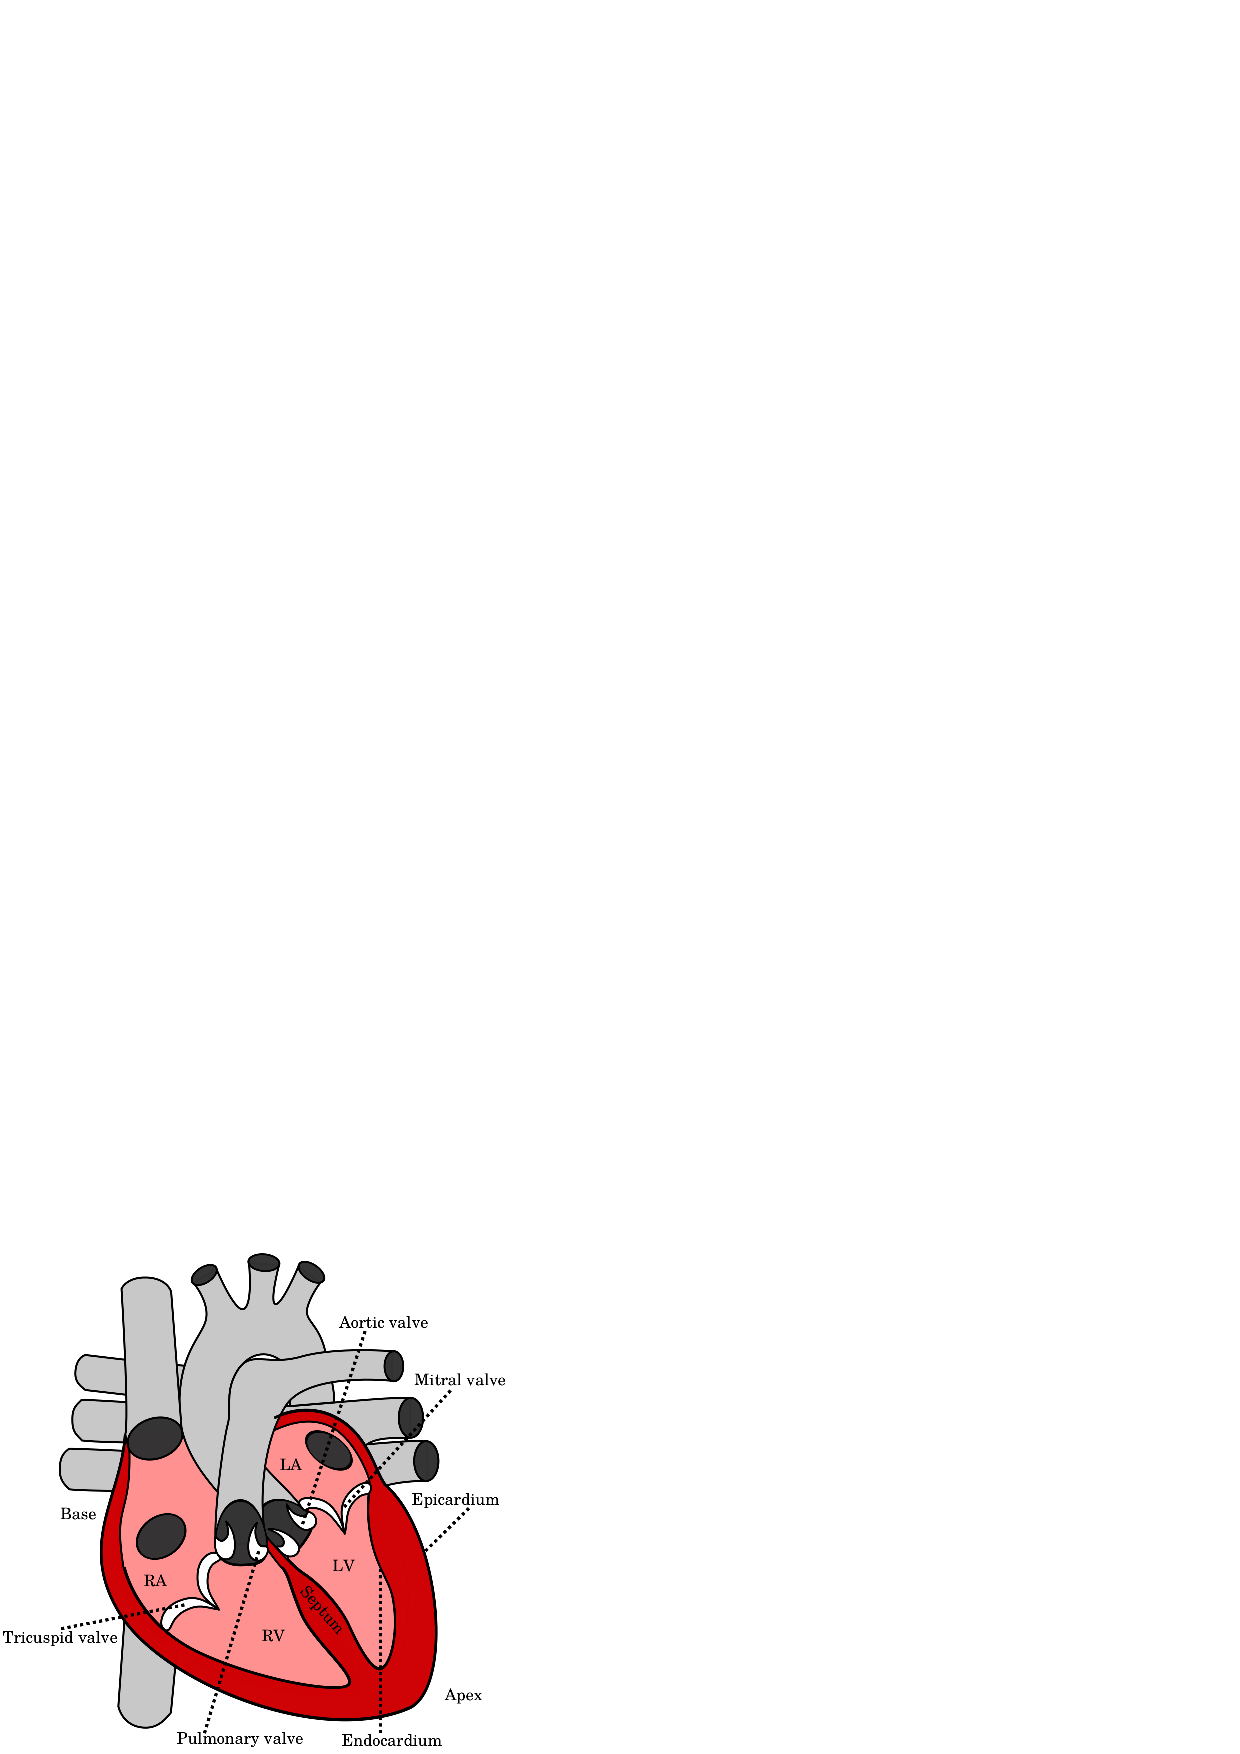
\includegraphics[width=0.7\textwidth]{chapters/introduction/figures/heart_anatomy.pdf}
\caption{The heart anatomy. (Adapted and modified from Wapcaplet in Sodipodi).}
\label{fig:heart_anatomy}
\end{figure}


Deoxgenated blood is transported from the body trough the veins and to
the right atrium (RA). From the RA, blood flows to the right ventricle
(RV), before it is sent through the the pulmonary ateries(PA) and to the
lungs, where the bloods gets oxygenated. From the lungs, the blood
travels trough the pulmonary veins to the left atrium (LA), and
finally to the left ventricle (LV), before is is sent out to the body
again trough the aorta (Ao). A schamtic view of the blood flow
through the body is shown in Figure ~\ref{fig:heart_anatomy}

The flow from one chamber to another is driven
by pressure gradients, that is blood flows from regions with higher
pressure to regions with lower pressure. Consequently, the lowest
pressure is found in the veins entering the heart, and the highest
pressure is found in the left ventricle.

The heart itself is located approximately in the center of the chest
with the \emph{apex} of heart angled down towards the left of the
body, and the \emph{base} located just behind the breastbone.



\subsection{Myocardial structure and morphology}

Starting form the outside of the heart we have the \emph{pericardium},
the \emph{epicardium}, the \emph{myocardium} and the \emph{endocardium}. 
The endo- and epicardium are respectively the inner and outer layers of the
myocardium, which is the cardiac muscle cells.

The myocardium is made up by individual cardiac muscle cells, or
cardiac myocytes which branch and join neighbouring cell, and form a
complicated fibrous network which is often referred to as a
\emph{functional syncytium} meaning that the number of active muscle
fibers cannot be varied from beat to beat. 


Each myocyte is composed of bundles of myofibriles, which again
contain \emph{myofilaments}. The myofilaments cosists of a repeated pattern
of lines and bands which can be seen as a collection of individual
contractile units called \emph{sarcomeres}. A simple sketch of a
sarcomere is shown in Figure \ref{fig:sarcomere}.

\begin{figure}[htbp]
  \centering
    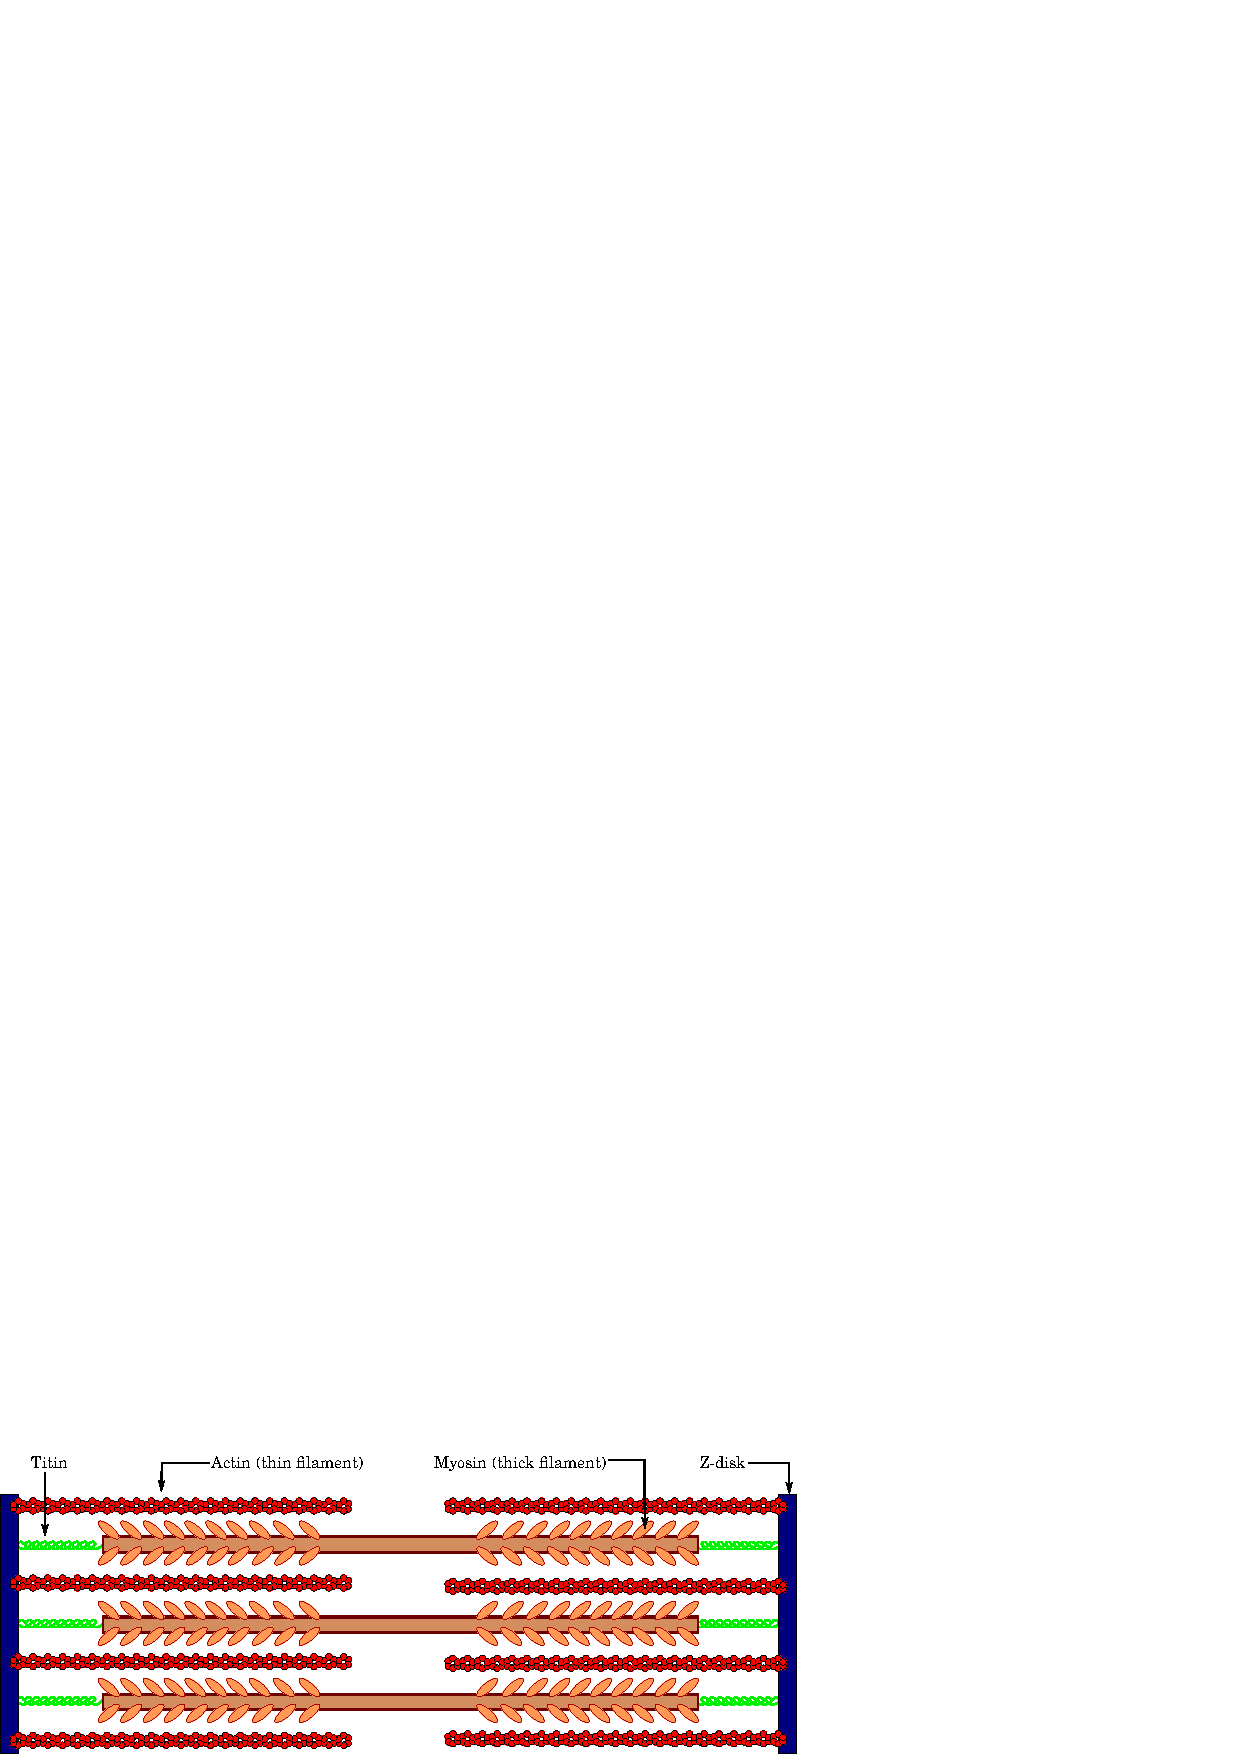
\includegraphics[width=1.0\textwidth]{chapters/introduction/figures/Sarcomere.png}
\caption{Illustration of the sarcomere structure.}
\label{fig:sarcomere}
\end{figure}

These sarcomeres are composed thick and thin filaments that slides
back and forth when the muscle contract or relaxes. For that reason we
also refer to this model as the sliding-filamen model. 
The thin filaments are made up by a protein called \emph{actin} while
the thick filaments are made up by a protein called \emph{myosin}.
In order for the muscle to contract, calcium enters the cell after a
triggered action potential. These calcium ions binds to a complex called
troponin C located at the thin filments, which then exposes the actin to the
myosion head. When myosin binds to actin we say that a
\emph{cross-bridge} is formed between the thin and thick
filments. Now several models exist for the crossbridge cycle that
constitutes the sliding filament theory, but main steps includes the
use of ATP in order to trigger the \emph{power stroke} which makes the 

\subsection{Passive and Active properties of the myocardium}
The myocardium is composed by small blood vessels that supply the
myocardial cells with oxygen. When the myocardium contracts this
perfused blood is then squeezed out, resulting in an overall loss of
volume. Such materials are referred to as compressible. When the
volume are preserved we refer to the material as incompressible.



\begin{figure}[htbp]
  \centering
    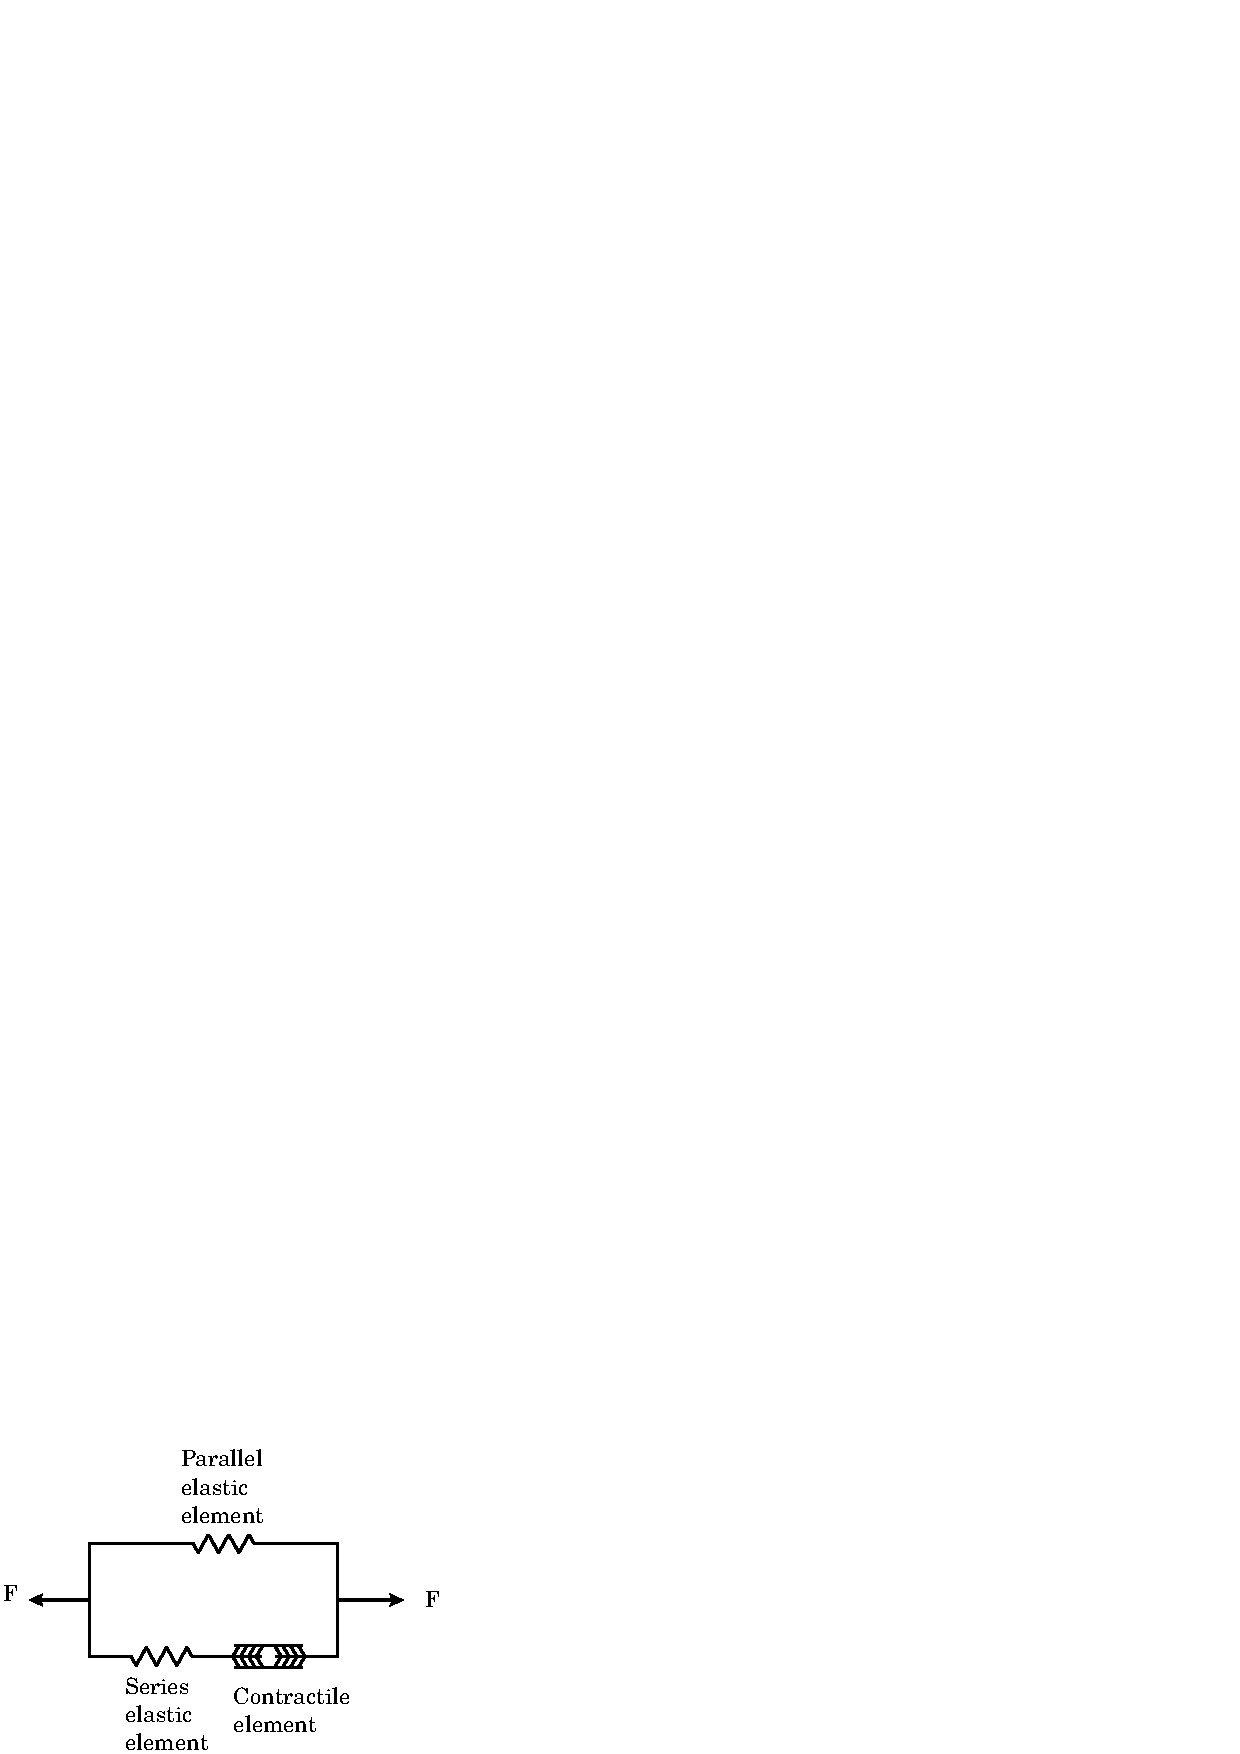
\includegraphics[width=0.5\textwidth]{chapters/introduction/figures/Hill_muscle_model.pdf}
\caption{The classical three-element Hill muscle model with one
  contractile element and two non-linear springs, one arranged in
  series and one parallel. }
\label{fig:hill_muscle_model}
\end{figure}



\subsection{Ventricular pumping function}
\label{sec:ventricular_pumping_function}
The left ventricle is by far the most studied chamber of the heart,
mainly because this is the chamber responsible for ejecting blood into the
body and therefore a diseased left ventricle could be fatal. A heart
beat can be described in many ways. One way is by looking at the
electrical propagation of current that travels through the heart and
activates the myocardium, leading to contraction. Such a diagram in
known as the \emph{electrocardiogram} (ECG). Another way to descrive
the cardiac cycle is by means of the LV pressure and volume. Plotting
the LV volume on the $x-$axis and the LV pressure on the $y-$axis
provides an intuitive representaion of the cardiac cycle known as the
\emph{PV-loop}, see Figure \ref{fig:pv_loop}.



\begin{figure}[htbp]
  \centering
    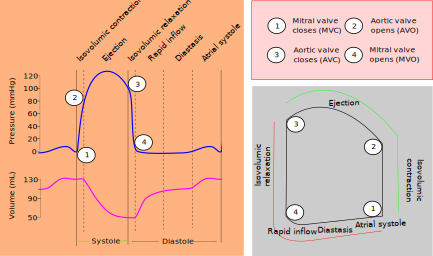
\includegraphics[width=0.8\textwidth]{chapters/introduction/figures/cardiac_cycle.png}
\caption{Showing the relation between pressure and volume in the left
  ventricle during the cardiac cycle, which the different phases and
  valvular events marked. To the left we show the a reduced version of
the classical Wiggers diagram with pressure and volume plotted against
time on the $x-$axis. To the right we show the pressure volume loop
with volume plotted on the $x-$axis and pressure on the $y-$axis. }
\label{fig:pv_loop}
\end{figure}



\subsection{Frank-Starling Mechanism and the Starling curve} 
The end diastolic pressure volume relationship (EDPVR), relates the end
diastolic volume to the end diastolic pressure. Simlarly the end
systolic pressure volume relationship (ESPVR) relates the end systolic
volume to the end systolic pressure. The Frank-Starling relationship,
relates the EDPVR to the ESPVR. The law states that the stroke volume
increases in response to and increase in end diastolic volume (as long
as the sarcomeres are working on the acending limb, which is usually
the case). This allows the cardiac output to be synchronized with the
venous return and blood supply without depending upon external
regulation.
The Starling Curve is a plot of the ESPVR - EDPVR, showing that the
output increases up to some maximum (at the acending limb). Thereafter
it decreases on the decending limb. If the sarcomeres works on the
decending limb, the heart would dilate and become weakend.

\subsection{Myocardial Contractility}

Contractility can be seen as the manifestation of all the factors that
influence the interactions between the contractile proteins.
One simple definitions is \emph{myocardial sontractility is the
  ability of the heart to do work}. A change in myocardial
contractility can be seen if there is a change in ejection which is
not caused by changes in the initial fiber lenght (ED). If the end
diastolic volume remains the same, but the stroke work changes there
is a change in contractility.

% Under normal circumstances, the myocardial cells generate less than
% half the of their maximal contractility. One could increase the
% contractility by providing more calcium to the cells.


In order to find a suitable idex for myocardial contractility we take
step back and consider Hills postulate: \emph{the ``active points'' of
  muscle can exist in two states: 1. active points are maintaining
  tension, 2. the active points are participating in a chemical
  reaction.} 
If the muscle is presented with a heavy load, developed tesion is
high, shortening velocity is low and the load is only moved a short
distance. In this case the active points are holding tesion.
On the other hand, if the muscle is presented with a light load, the
shortening velocity is high and the load is moved a longer
distance. In this case more of the active points are participating in
chemical reactions. 
In both cases, the contractility might be the same which is why we
need a load independent measure of contractility.
Looking at the force-velocity relationship we can say that the maximum
force (tesion) is acheived when all the active points are holding
tesion ($P_0$). $P_0$ is proportional to the number of active
cross bridges.
Similarly, the maximum velocity is acheived when all
the active points are participating in a chemical reaction
($V_{\text{max}}$). $V_{\text{max}}$ reflects the maximal rate of
cross bridge cycling. 
This is explained by the Hill eqation, which
relates the force to velocity, and the interects are $P = P_0, (V = 0)$
and $V = V_{\text{max}}, (P = 0)$. This is very difficult to meause in
cardiac cells because cariac muscle cells are not tentanized.

The most commonly used index of contractility was formalized
\cite{sagawa1977end} using a time varying elastance model, which
states that at any point in the cardiac cycle the pressure and volume
are linearly related by the time-varying elastance, or formally:
\begin{align}
  P(t) = E(t)( V(t) - V_0 ).
  \label{eq:time_varying_elastance}
\end{align}
Here $P$ is the endocardial pressure, $V$ the cavity volume, $E$ the
time-varying elastance, and $V_0$ the volume axis intercept. This
model


\subsection{Summar of Cardiac Physiology}
The multiscale and multiphysics phenomena governening the mechanics of
the heart is complex. How the molecular dynamics should be coupled to
the electrophysiology at the cellular level, how the electrophysiology
should be coupled to the mechanics at the organ level and what type of
feedback mechanisms that should be included is far from fully
understood. In this thesis we limit ourself to the study of what is
happending on the organ level.


%%% Local Variables:
%%% mode: latex
%%% TeX-master: "../../main"
%%% End:
